\documentclass[12pt,a4paper]{article}
\usepackage{graphicx}
\usepackage{amsmath}
\usepackage{amsthm}
\usepackage{tikz}

\begin{document}

\section{The Mauna Loa $CO_2$ Concentration}

\subsection{Problem statement}

In 1958, Charles David Keeling (1928-2005) from the Scripps Institution of Oceanography began recording $CO_2$ concentrations in the atmosphere at an observatory located at about 3,400 m altitude on the \textbf{Mauna Loa Volcano} on Hawaii Island. 

The location was chosen because it is not influenced by changing $CO_2$ levels due to the local vegetation and because prevailing wind patterns on this tropical island tend to bring well-mixed air to the site. While the recordings are made near a volcano (which tends to produce CO), wind patterns tend to blow the volcanic CO away from the recording site. 

Air samples are taken several times a day, and concentrations have been observed using the same measuring method for over 60 years. In addition, samples are stored in flasks and periodically reanalyzed for calibration purposes. The result is a data set with very few interruptions and very few inhomogeneities.

Let $C_i$ be the average $CO_2$ concentration in month $i$ ($i=1,2, ...$, counting from March 1958). We will look for a description of the form:
\begin{equation}
	C_i = F(t_i) + P_i + R_i
\end{equation}
where:
\begin{itemize}
	\item $F: t \to F(t)$ accounts for the long-term trend;
	\item $t_i$ is time at the middle of the $i^{th}$ month, measured in \textbf{fractions of years} after Jan 15, 1958. Specifically, we take $t_i = \frac{i+0.5}{12}$ where $i=0$ corresponds to Jan, 1958, adding $0.5$ is because the first measurement is halfway through the first month;
	\item $P_i$ is periodic in $i$ with a fixed period, accounting for the seasonal pattern;
	\item $R_i$ is the remaining residual that accounts for all other influences.
\end{itemize}

The goal of is to \textbf{fit the data and understand its variations}.

\paragraph{Note} The decomposition is meaningful only if the range of $F_i$ much larger than the amplitude of the $P_i$ and this amplitude in turn is substantially larger than that of $R_i$ .

\subsection{Trend estimation}

In this section we fit three polynomial trends of order $n=1, 2, 3$ to the $CO_2$ concentration data. 

\begin{align}
	F_1 (t) &\sim \alpha_0 + \alpha_1 \\
	F_2 (t) &\sim \beta_0 + \beta_1 t + \beta_2 t^2 \\
	F_3 (t) &\sim \gamma_0 + \gamma_1 t + \gamma_2 t^2 + \gamma_3 t^3
\end{align}

Before fitting these models, we perform 80:20 train to test partition. This way we can measure performance using RMSE and MAPE on both train and test sets, and detect potential overfitting.

\begin{figure}[h!]
	\centering
	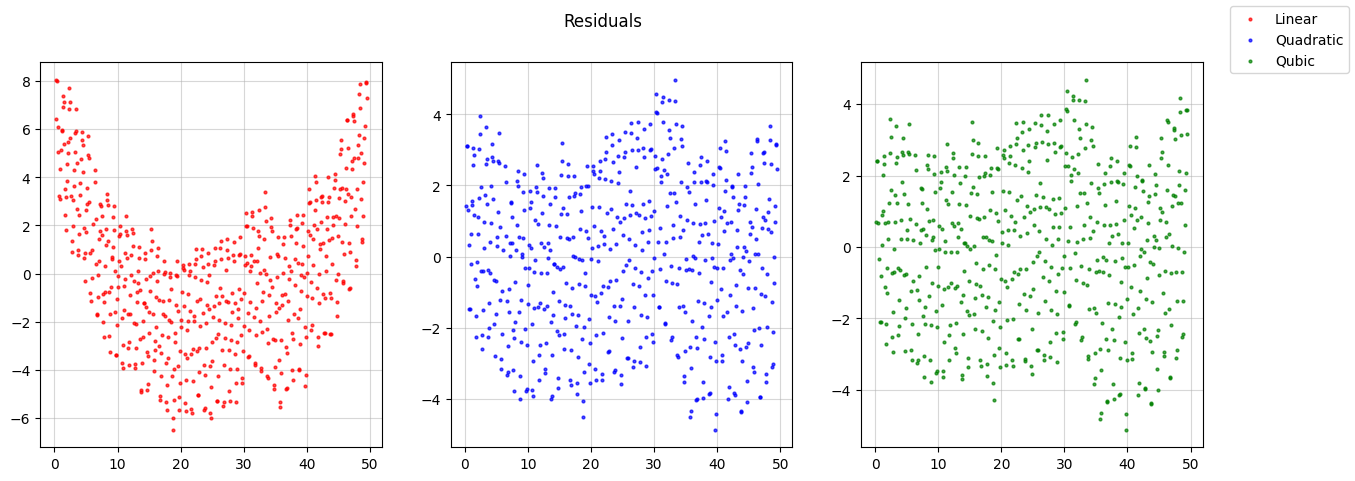
\includegraphics[width=0.9\textwidth]{figures/residuals.png}
	\caption{Residuals for each trend model}
\end{figure}

When we fit the linear model, on the residual plot we can clearly see U-shaped figure, which implies that there is a quadratic component. Residual almost doesn't change for quadratic and qubic models. 

\begin{figure}[h!]
	\centering
	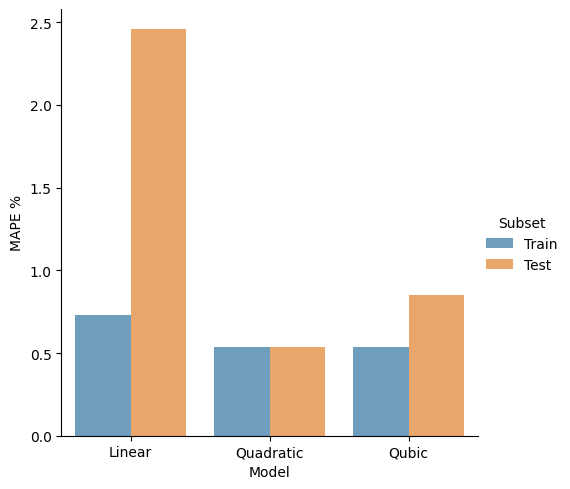
\includegraphics[width=0.4\textwidth]{figures/performance.png}
	\caption{Model performance measured with MAPE}
\end{figure}

Also, on the MAPE bar chart, we notice that qubic model overfits the data. Thus, it's suggested to use quadratic $F_2$ as the trend model.

\subsection{Seasonality}

Let's compare ACF for $C_i$, and for $C_i - F_2 (t_i)$ i.e. after we have removed the trend. 

\begin{figure}[h!]
	\centering
	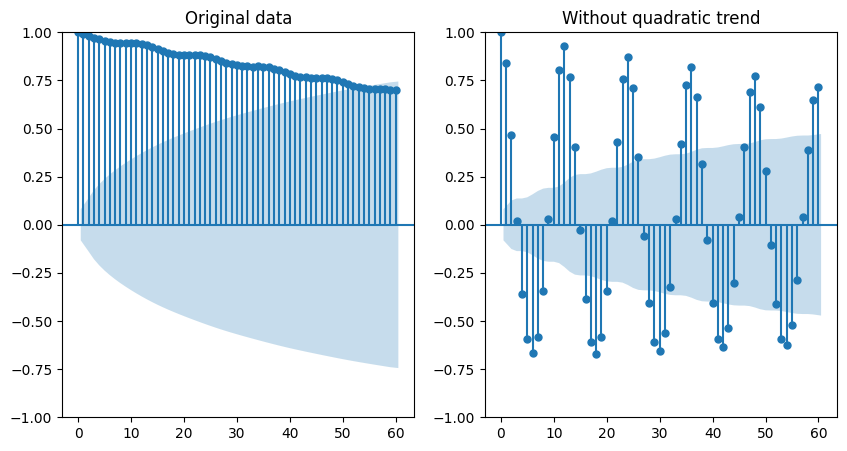
\includegraphics[width=0.8\textwidth]{figures/auto_correlation_trend.png}
	\caption{ACF before and after removing trend}
\end{figure}

We see that there is a clear periodic pattern on the ACF plot for $C_i - F_2 (t_i)$. 

The easiest way to extract the periodic component is to collect all the residuals (from removing quadratic trend $F_2$) for each month over the years and average them to get one data point for respective month. Then, the collection of these points can be interpolated to form a periodic signal, that is:
\begin{equation}
	P_{i+12} = P_i
\end{equation}

\begin{figure}[h!]
	\centering
	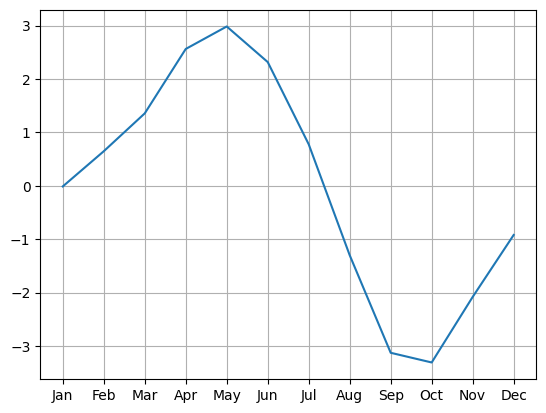
\includegraphics[width=0.5\textwidth]{figures/periodic_part.png}
	\caption{Periodic component of $CO_2$ concentration}
\end{figure}

\subsection{Final decomposition and results}

Comparing prediction with the test data, the prediction diverges as we go further in time.

\begin{figure}[h!]
	\centering
	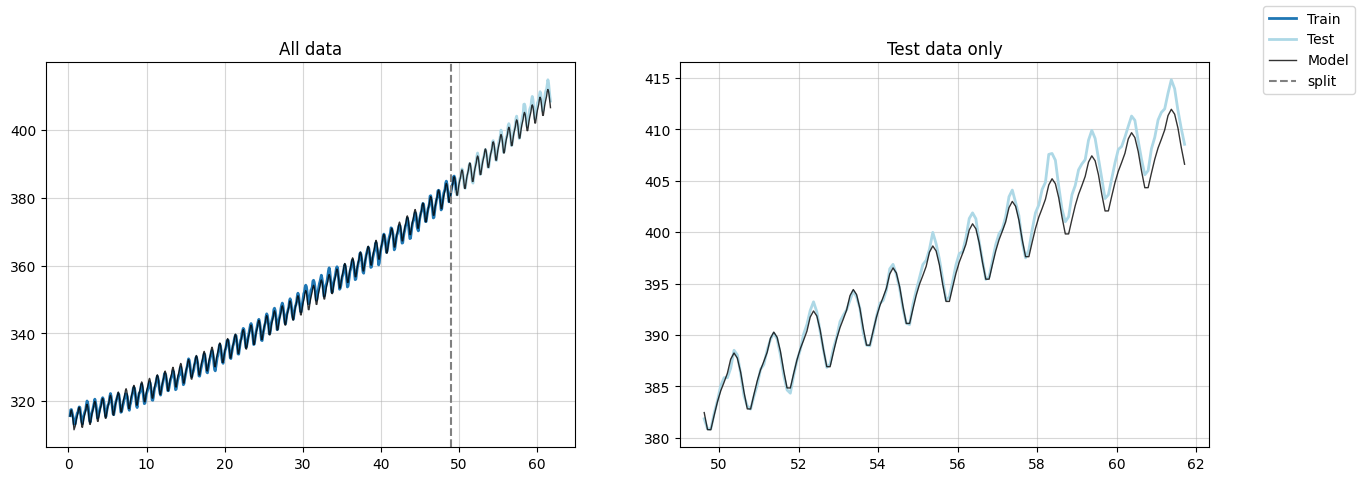
\includegraphics[width=\textwidth]{figures/co2_prediction.png}
	\caption{Real $CO_2$ concentration vs prediction}
\end{figure}

Final model performance measured by RMSE and MAPE is more than two times better, than for the previous model with deterministic quadratic trend $F_2$. This tells us the significant role of periodic component in $CO_2$ concentration.

\begin{table}[h!]
	\begin{tabular}{|l|l|l|}
		\hline
		Model				& RMSE & MAPE \\ \hline
		$F_2 (t_i)$ 		& 2.508 & 0.534 \% \\ \hline
		$F_2 (t_i) + P_i$ 	& 1.153 &  0.21 \% \\ \hline
	\end{tabular}
	\centering
	\caption{Performance comparison}
\end{table}

To show that the decomposition is meaningful, let's compare the range of values $\max - \min$ for each part of the decomposition of the training set.

\begin{table}[h!]
\begin{tabular}{|l|l|}
	\hline
	Ratio 			& Value \\ \hline
	$F$ to $P_i$ 	& 10.99 \\ \hline
	$P_i$ to $R_i$  & 1.64 \\ \hline 
\end{tabular}
\centering
\caption{Ratio of amplitudes of decomposition components}
\end{table} 

We can also look at the ACF plot for our final residual. If we compare it with the previous such plot, the ACF drops to zero relatively quickly, but still doesn't fully support the stationarity hypothesis. Despite the fact we have fitted two main components (trend + seasonality), and the model seems to satisfy our definition of meaningfulness, and the mean $\bar{R_i} = -1.045 \cdot 10^{-14} \approx 0$, there could still be a \textbf{certain external regressor} which we weren't able to fit. 

\begin{figure}[h!]
	\centering
	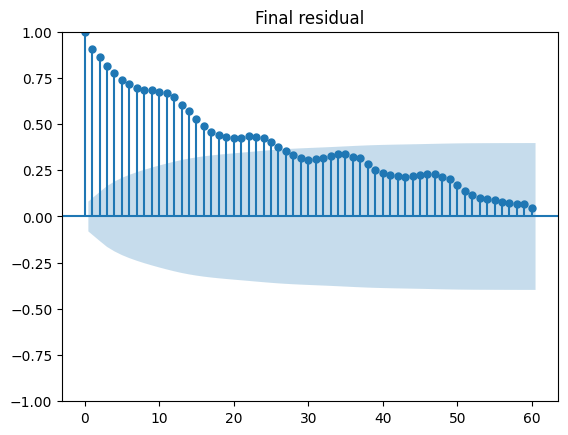
\includegraphics[width=0.8\textwidth]{figures/final_acf.png}
	\caption{ACF for $R_i$ residual}
\end{figure}


\end{document}